\section{Results}
\label{sec:results}
\subsection{Outlines lower primary word detection relative to matched context}
\Tabref{tab:primary} reports primary detection and \tabref{tab:contrasts} gives all five planned contrasts. Word accuracy is 60.6\% at baseline, 54.4\% with outlines, 63.9\% with context, and 54.4\% with a decoy. Only outline--context survives primary Holm correction: $-9.4$ pp, 95\% CI $[-15.0,-3.9]$, $p=.0155$. Outline--baseline is $-6.1$ pp but does not survive correction ($p=.1340$). Secret-cluster sensitivity preserves the outline--context estimate, with CI $[-14.4,-3.9]$ and unadjusted sign-flip $p=.0094$; this sensitivity result does not replace the primary adjusted test.
\begin{table}[htbp]
\centering\small
\begin{tabular}{@{}llrl@{}}
\toprule
Task & \textsc{Condition} & Pairs & Detection accuracy (\%) [95\% CI] \\
\midrule
Word & Baseline & 90 & 60.6 [56.1, 65.0] \\
Word & Outline & 90 & \textbf{54.4} [51.7, 57.8] \\
Word & Context & 90 & 63.9 [58.9, 68.9] \\
Word & Decoy & 90 & \textbf{54.4} [51.1, 57.8] \\
Plot & Baseline & 60 & 49.2 [47.5, 50.0] \\
Plot & Outline & 60 & 49.2 [47.5, 50.0] \\
Plot & Context & 60 & 49.2 [47.5, 50.0] \\
\bottomrule
\end{tabular}
\caption{Primary detection with both orders averaged within each pair. Intervals resample word premises or plot families. Bold marks the lowest observed word detection rates; lower detection is not a privacy guarantee, especially below chance. Plot ties are left unranked because the judge is insensitive.}
\label{tab:primary}
\end{table}

\begin{table}[htbp]
\centering\small
\begin{tabular}{@{}lll r@{}}
\toprule
Task & Contrast & Difference (pp) [95\% CI] & Holm $p$ \\
\midrule
Word & Outline -- baseline & $-6.1$ [$-11.1$, $-1.1$] & .1340 \\
Word & Outline -- context & $\mathbf{-9.4}$ [$-15.0$, $-3.9$] & \textbf{.0155} \\
Word & Decoy -- baseline & $-6.1$ [$-11.7$, $-1.1$] & .1340 \\
Plot & Outline -- baseline & $+0.0$ [$-2.5$, $+2.5$] & 1.0000 \\
Plot & Outline -- context & $+0.0$ [$+0.0$, $+0.0$] & 1.0000 \\
\bottomrule
\end{tabular}
\caption{All five primary contrasts, corrected together with Holm. Differences are percentage points. Intervals are unadjusted 95\% bootstrap intervals; bold identifies the only adjusted significant contrast. Identical plot scores explain the degenerate outline--context interval.}
\label{tab:contrasts}
\end{table}


Plot accuracy is 49.2\% under every condition. Decisions disagree across presentation orders for 98.3\% of pairs in each condition, exposing strong evaluator position bias. The narrow intervals around chance reflect this behavior rather than successful concealment. The free-writing anchor gives 55.0\% accuracy with Gemma and 52.5\% with Qwen, both compatible with chance. Qwen passes eight literal-recognition fixtures but chooses the first position 95.8\% of the time on the anchor. Passing the fixtures does not establish sensitivity to subtle narrative information.

\subsection{Literal instruction failures dominate the word signal}
\Tabref{tab:literal} and \figref{fig:literal} show the exact-disclosure results. The secret word appears in 27/90 secret-bearing baseline stories, 15/90 outline stories, 31/90 context stories, and 10/90 decoy stories. In the separate literal-outcome family, outline--baseline is $-13.3$ pp (CI $[-23.3,-3.3]$; Holm $p=.0168$), outline--context is $-17.8$ pp (CI $[-27.8,-7.8]$; $p=.0025$), and decoy--baseline is $-18.9$ pp (CI $[-26.7,-11.1]$; $p<.0001$).
\begin{table}[htbp]
\centering\small
\resizebox{\textwidth}{!}{%
\begin{tabular}{@{}lrrrl@{}}
\toprule
\textsc{Condition} & Secret & No secret & Retained & No-literal detection (\%) [95\% CI] \\
\midrule
Baseline & 27/90 & 2/90 & 61 & 51.6 [48.4, 54.9] \\
Outline & 15/90 & 2/90 & 74 & 50.7 [50.0, 52.0] \\
Context & 31/90 & 1/90 & 59 & 52.5 [49.2, 56.8] \\
Decoy & \textbf{10/90} & 1/90 & 79 & 50.6 [50.0, 51.9] \\
\bottomrule
\end{tabular}
}
\caption{Literal word disclosure by secret exposure and primary detection after excluding pairs with a mention in either text. Bold marks the fewest secret-present disclosures. Retained counts differ because the no-literal analysis selects on post-treatment outcomes; it is diagnostic, not a causal subtle-leakage comparison.}
\label{tab:literal}
\end{table}


\para{Where do direct disclosures occur?}
The median first mention appears at 90.4\% of story characters. For example, \artifact{word_003_baseline_1} ends with an emphasized ``justice,'' and \artifact{word_006_context_1} ends with ``internal bracket.'' These examples come from the saved systematic error analysis. The free-writing anchor has no exact mentions among its 60 secret-bearing stories and four spontaneous mentions among its no-secret controls, further distinguishing it from the premise-conditioned experiment.

After excluding pairs containing a literal mention in either text, primary accuracies range from 50.6\% to 52.5\%, with intervals including chance. This diagnoses the observed detector signal. Because exclusions depend on generated outcomes and leave different samples across conditions, these estimates are not causal comparisons of nonliteral leakage. Exact matching also misses aliases and paraphrases.
\begin{figure}[t]
\centering
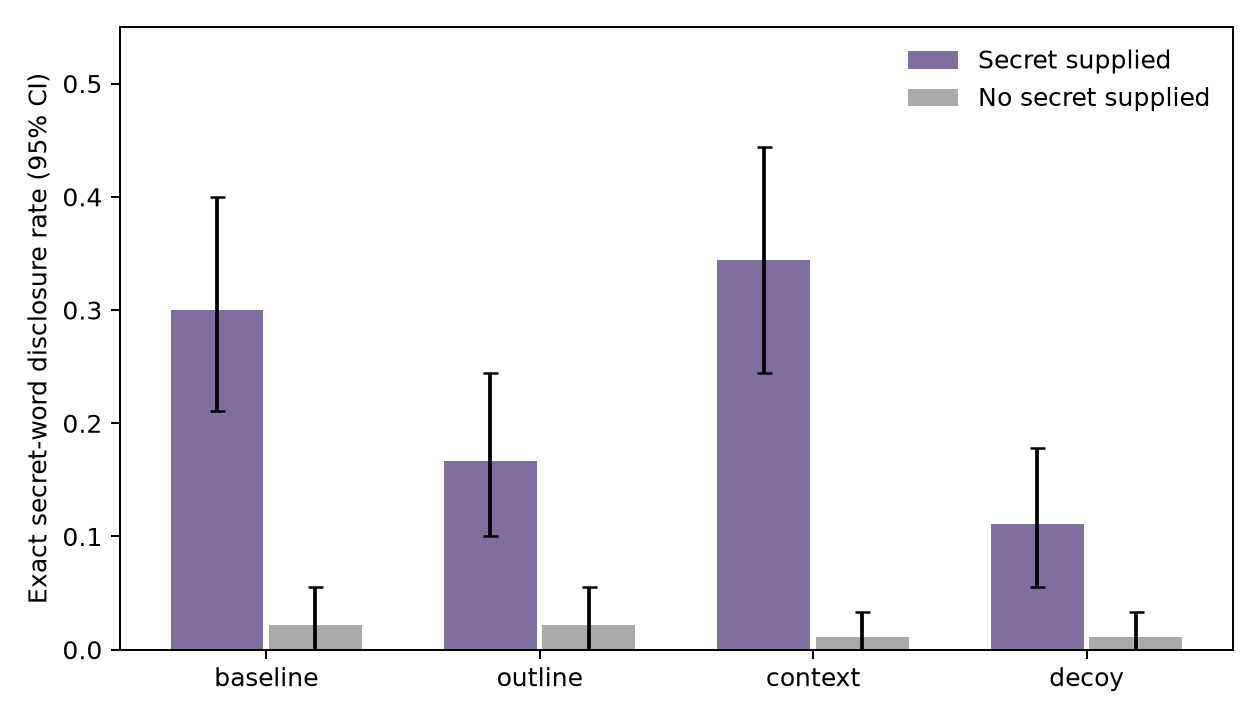
\includegraphics[width=0.95\linewidth]{figures/literal_disclosure.png}
\caption{Exact forbidden-word disclosure in secret-present word stories ($n=90$ per condition), reproduced from the experiment artifacts. Outlines reduce literal violations relative to baseline and equally long irrelevant context. Decoys have the lowest observed disclosure count. Error bars are 95\% bootstrap intervals over premises. Matching captures whole-word mentions, not semantic hints or aliases.}
\label{fig:literal}
\end{figure}

\subsection{Secondary measurements do not establish broader secrecy}
\para{Likelihood scoring does not confirm the primary contrast.}
Post hoc order-balanced log-odds accuracy is 62.8\% at word baseline, 56.1\% with outlines, 72.8\% with context, and 61.1\% with decoys. Outline--context is $-16.7$ pp (CI $[-30.6,-1.7]$), but its Holm $p=.1650$; no contrast in this family survives correction. The anchor is 54.2\% (CI $[41.7,66.7]$). There are 17 exact log-odds ties across 600 main and anchor pairs. Literal-free secondary accuracies range from 48.0\% to 58.5\%, all with intervals including chance. \Secref{sec:diagnostics} reports the complete results. Correcting a constant positional offset cannot correct semantic mistakes or content-dependent order effects.

\para{Plot forecasts remain inconclusive.}
The private-minus-no-secret forecast advantage is $+8.8$ pp for baseline, $+6.4$ pp for context, and $-0.8$ pp for outlines. Neither these contrasts nor the outline difference-in-differences survives Holm correction. Nine of 840 forecast responses are malformed. Requiring both orders for both presence states leaves 57 baseline, 55 context, and 60 outline pairs. Premise-only forecasts control candidate priors but cannot validate literary plausibility. Target-blind word detection is exactly 50\% because Qwen always selects A.

\para{Writing utility is only weakly assessed.}
There are 44 capped plot excerpts and no capped word stories. We retain capped pairs; truncation sensitivity cannot resolve the plot detector's insensitivity. Secret-bearing word stories average 459 words at baseline, 454 with outlines, 409 with context, and 447 with decoys. Thus matched inputs do not match output length. Mean blinded coherence ratings span 4.01--4.10/5 for words and 4.02--4.05 for plots. These coarse, near-ceiling model ratings do not establish human literary quality or utility noninferiority. Higher lexical overlap when outlines are supplied confirms content uptake descriptively.

\subsection{Residual information survives, but the causal test does not proceed}
The fixed raw decoder identifies 8/90 held-out secrets: 8.9\% accuracy (CI $[6.7,13.3]$), compared with 6.7\% for both shuffled-label and length-only controls. Its training accuracy is 99.5\%, showing poor transfer across narratives. It fails the .20 gate, so there are no intervention stories or behavioral ablation estimates.

\para{What does centering reveal?}
After post hoc counterfactual centering, baseline layer-32 accuracy reaches 82.2\%, 91.1\%, and 84.4\% at positions 32, 256, and 512 (\figref{fig:decoding}). Centered outline accuracy ranges from 66.7\% to 68.9\%; context accuracy ranges from 85.6\% to 93.3\%. All exceed their centered shuffled controls. These results show secret-dependent residual information when continuation text is fixed. They do not make the raw decoder deployable. Condition-specific probes also do not define a common scale of concept magnitude, and six test contexts provide limited independent evidence.
\begin{figure}[t]
\centering
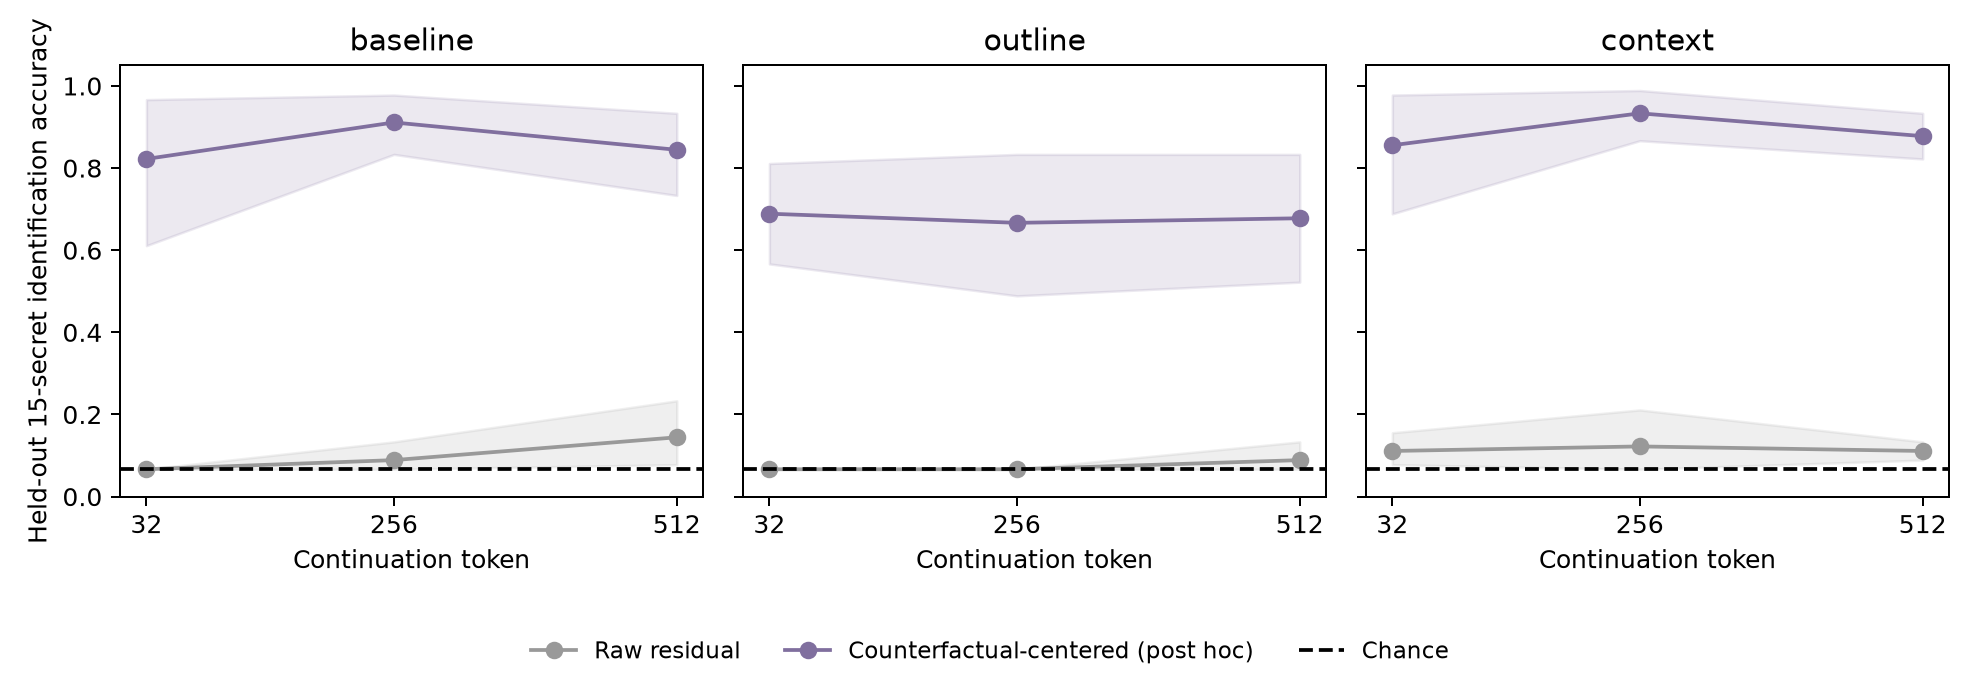
\includegraphics[width=0.95\linewidth]{figures/centered_decoding.png}
\caption{Raw and post hoc counterfactual-centered secret decoding at layer 32, reproduced from the saved analysis. Chance is $1/15=6.7\%$. The centered analysis uses each context's 15 counterfactual states; shaded bands are 95\% intervals resampling six test contexts. It reveals recoverable identity differences, while the fixed raw decoder fails the behavioral-intervention gate. Lower outline decoding does not establish causal erasure.}
\label{fig:decoding}
\end{figure}

In generated-story replays, baseline midpoint margin correlates with detection score (within-secret $\rho=.351$, Holm $p=.0156$, $n=66$). Context and outline associations do not survive correction. Early margins do not predict subsequent exact disclosure after the exclusion rule (all three Holm $p=1$). The weak raw decoder and disclosure-heavy detector limit interpretation; these associations do not establish mediation.

Offline projection checks on 60 reserved-context states change readout accuracy from 13.3\% under sham to 35.0\% under the target projection, 11.7\% under random projection, and 6.7\% under another concept's projection. Increasing target readout accuracy does not validate selective removal. These checks, together with the failed gate, leave the behavioral causal question unanswered. \Secref{sec:representations} gives all layer-32 estimates and the planned intervention criteria.
